%% LyX 2.3.6.1 created this file.  For more info, see http://www.lyx.org/.
%% Do not edit unless you really know what you are doing.
\documentclass[11pt,twoside,english]{scrreprt}
\PassOptionsToPackage{natbib=true}{biblatex}
\usepackage{lmodern}
\usepackage[T1]{fontenc}
\usepackage[latin9]{inputenc}
\usepackage[a4paper]{geometry}
\geometry{verbose,tmargin=30mm,bmargin=30mm,lmargin=30mm,rmargin=15mm}
\pagestyle{empty}
\usepackage{color}
\usepackage{babel}
\usepackage{float}
\usepackage{textcomp}
\usepackage{bm}
\usepackage{amsmath}
\usepackage{amsthm}
\usepackage{amssymb}
\usepackage{graphicx}
\usepackage{setspace}
\setstretch{1.3}
\usepackage[unicode=true,pdfusetitle,
 bookmarks=true,bookmarksnumbered=false,bookmarksopen=false,
 breaklinks=false,pdfborder={0 0 0},pdfborderstyle={},backref=false,colorlinks=false]
 {hyperref}

\makeatletter

%%%%%%%%%%%%%%%%%%%%%%%%%%%%%% LyX specific LaTeX commands.
%% Because html converters don't know tabularnewline
\providecommand{\tabularnewline}{\\}
\floatstyle{ruled}
\newfloat{algorithm}{tbp}{loa}[chapter]
\providecommand{\algorithmname}{Algorithm}
\floatname{algorithm}{\protect\algorithmname}

%%%%%%%%%%%%%%%%%%%%%%%%%%%%%% User specified LaTeX commands.
\usepackage{lipsum}

%\usepackage[left,modulo]{lineno}
%\usepackage[left]{lineno}
%\usepackage{scrlayer-scrpage}
\usepackage[automark,headsepline]{scrlayer-scrpage}

%\usepackage{helvet}
%\renewcommand{\familydefault}{\sfdefault}
\usepackage{empheq}

\makeatother

\usepackage{listings}
\usepackage[style=numeric]{biblatex}
\renewcommand{\lstlistingname}{Listing}

\addbibresource{library.bib}
\begin{document}

%\addtokomafont{disposition}{\rmfamily} %Changes the disposition font to Times
%\setkomafont{disposition}{\bfseries} 
%\renewcommand{\familydefault}{\sfdefault} % change all font from default Times to sans-serif

\clearpairofpagestyles

\newgeometry{ a4paper, top=25mm, bottom=25mm, inner=25mm, outer=25mm }

\begin{titlepage}
\begin{flushleft}

\includegraphics[width=0.25\paperwidth]{graphics/schoolLogo}
\par\end{flushleft}

\vspace*{0.1\textheight}

\noindent \begin{center}
\textsf{Master Thesis}
\par\end{center}

\vspace{0.03\textheight}

\begin{spacing}{1.4}
\noindent \begin{center}
\textsf{\textbf{\huge{}Making thesis reports great again}}{\huge\par}
\par\end{center}
\end{spacing}

\vspace{0.03\textheight}

\begin{singlespace}
\noindent \begin{center}
Your Name\vspace{0.03\textheight}
\par\end{center}
\end{singlespace}

\begin{center}
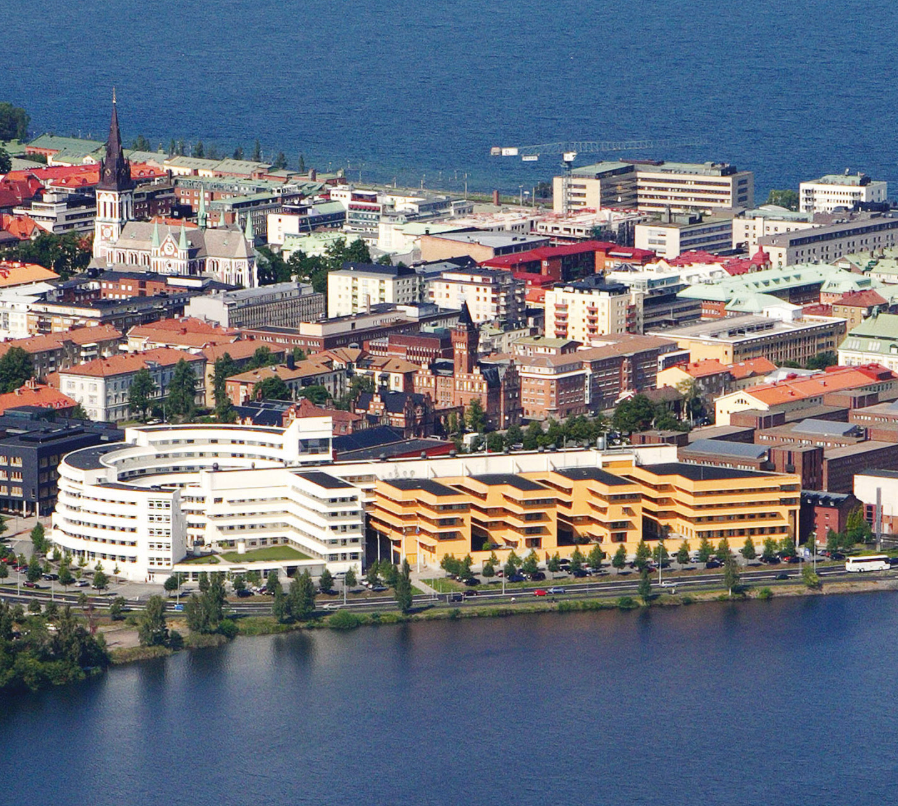
\includegraphics[width=0.35\paperwidth]{graphics/jupic}
\par\end{center}

\vspace{0.1\textheight}

\begin{center}
\par\end{center}

\vfill{}

\noindent \begin{flushleft}
\textsf{J�nk�ping University}\\
\textsf{School of Engineering }\\
\textsf{Department of Product Development \textbullet{} June 2019}
\par\end{flushleft}

\end{titlepage}

\clearpage{}

\KOMAoptions{headsepline=false}

\null

\vfill{}

\noindent This thesis has been carried out at the School of Engineering,
J�nk�ping University, in the subject area Mechanical Engineering.
The authors answer themselves for opinions, conclusions and results.

\noindent %
\begin{minipage}[t]{0.15\columnwidth}%
\noindent Examiner:

Supervisors:\\
\\
Scope:\\
Date:%
\end{minipage}%
\begin{minipage}[t]{0.8\columnwidth}%
\noindent Keneth Salamandersson

Pontiak Johansson, F�retag AB\\
Dalibor Chennysson, J�nk�ping University\\
15 credits\\
2019-06-04%
\end{minipage}

\clearpage{}

\clearpairofpagestyles
\cfoot[\pagemark]{\pagemark}
%\lehead{\headmark}
%\rohead{\headmark}
\chead{\leftmark}
%\lehead{\leftmark} %left even head. leftmark is the chapter name
%\lohead{\leftmark}
%\rehead{\rightmark} %right even head. rightmark is the section name
%\rohead{\rightmark}

\KOMAoptions{headsepline=true}


\newgeometry
{ 
a4paper, 
top=30mm, 
bottom=30mm, 
inner=20mm, 
outer=20mm 
} 

\pagenumbering{roman} 

%\linenumbers 

\chapter*{Abstract}

\addcontentsline{toc}{chapter}{Abstract}

\textbf{What is an Abstract?}

The abstract is the second most read part of your thesis (after the
title page). As such, it needs to work for a wider audience than the
thesis itself who are often most interested in your results. The abstract
should be possible to read independently of the thesis itself.

\textbf{Purpose and scope}

What is the main message of your thesis? And how far do you investigate
this?

\textbf{Methods}

What did you do to get your results? (e.g. analyzed 3 articles, completed
a series of 5 experiments, interviewed 10 respondents)

\textbf{Results}

What answer was found to the research question? What did the study
find?

\textbf{Conclusion}

What are the larger implications of your findings, especially for
the purpose identified in step 1?

\textbf{Tips:}
\begin{itemize}
\item Emphasize the most important elements of the report
\item Use short sentences but vary sentence structure
\item Keep vocabulary as clear as possible e.g. explain terms / abbreviations
that might be unfamiliar to a wider audience
\item The abstract is usually the last part of the thesis to be written
\end{itemize}

\chapter*{Sammanfattning}

\addcontentsline{toc}{chapter}{Sammanfattning}

Same as abstract but written in swedish. Not needed at master level.

\chapter*{Preface}

\addcontentsline{toc}{chapter}{Preface}

Where and when was the thesiswork perfomed? What educational program
was finished with this thesis?

\noindent Thank all the supervisors, people that helped during the
work, family and friends.

\noindent Place and date

\noindent Authors Name

\tableofcontents{}

\chapter{Introduction}

\noindent \pagenumbering{arabic} 

\section{Background}

\subsection{Company AB}

Company ABwas founded in Sweden 1920 by some guy. For many years,
the company has provided important stuff to some industry with world
class technology of some system.

\lipsum[1-2]

\subsection{Some topic}

Look at this graph, see Figure \ref{fig:LookAtThisGraph}.
\begin{figure}[H]
\centering{}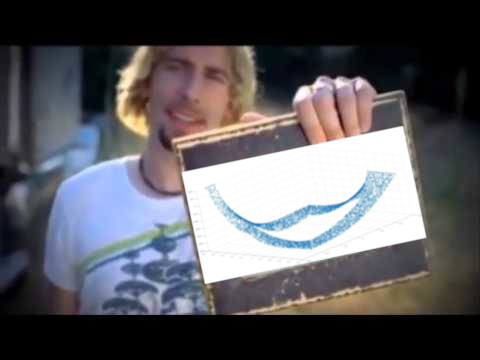
\includegraphics[width=0.6\paperwidth]{graphics/chad}\caption{Look at this graph\label{fig:LookAtThisGraph}}
\end{figure}

\pagebreak{}

\section{Problem Description}

\lipsum[1-2]

\pagebreak{}

\subsection{Requirements}
\begin{enumerate}
\item Requirement 1
\item Requirement 2
\end{enumerate}

\section{Purpose and Aim}

The purpose and aim of this thesis is to write a beautiful thesis.
The following issues will be answered throughout this report:
\begin{itemize}
\item Is this real life?
\item Or is this just fantasy??
\end{itemize}

\section{Delimitations}
\begin{itemize}
\item \lipsum[1-2]
\end{itemize}

\section{Outline}

The theoretical background in Chapter 2 presents relevant basic theories
to provide knowledge of how the concepts should be dimensioned, designed
and evaluated. Methods are presented in Chapter 3 with accompanying
simulation models. Evaluation and numerical results of the concepts
are presented in Chapter 4. Thorough analysis of the final concept
is located in Chapter 5. The report ends with discussion and conclusions
in Chapter 6.

\chapter{Theory}

\section{Connection Between Problem and Theories}

\begin{figure}[H]
\begin{centering}
\includegraphics[width=0.6\paperwidth]{\string"graphics/Problem and Theories\string".eps}\caption{Overview of which theoretical foundations contributed a solution to
the problem within this thesis}
\par\end{centering}
\end{figure}

\begin{itemize}
\item \lipsum[1-2]
\end{itemize}

\section{Some equations\label{sec:Fluid-Dynamics}}

Bernoulli\textquoteright s equation in fluid dynamics expresses the
energy of incompressible fluids i.e., the fluid density is constant
and in frictionless flow at the coordinate $s$. Daniel Bernoulli
stated, in such conditions, that the fluid pressure $p_{s}$, kinetic
energy $\frac{1}{2}\rho u_{s}^{2}$ and potential energy $\rho gz_{s}$
correlates. Bernoulli published his principle in his book Hydrodynamic
in 1738.\\
In incompressible fluid conditions, the total energy equation remains
constant according to equation \ref{eq:1PointFluid} \citealt{Storck2010}.

\begin{equation}
p_{s}+\frac{1}{2}\rho u_{s}^{2}+\rho gz_{s}=\mathrm{constant}\label{eq:1PointFluid}
\end{equation}

Due to \ref{eq:1PointFluid}, the energy at two points on a streamline
will be the same. The principle can be utilized by using two points
$1\:\&\:2$ on a streamline to extract unknown values according to
the equation \ref{eq: 2PointFluid}.

\begin{equation}
p_{1}+\frac{1}{2}\rho\bar{u}_{1}^{2}+\rho gz_{1}=p_{2}+\frac{1}{2}\rho\bar{u}_{2}^{2}+\rho gz_{2}\label{eq: 2PointFluid}
\end{equation}

If we assume the system is incompressible, if there is no change in
potential energy i.e. the relation of two points distance to a reference
level is zero and if no pressure drop is allowed, the kinetic energy
in point 1 must be larger than the kinetic energy in point 2 according
to the equation \ref{eq:BernoulliSimplified}.

\[
p_{2}\geq p_{1},
\]

\[
\Delta\rho gz=0,
\]

\[
\rho_{2}-\rho_{1}=0,
\]

\begin{equation}
p_{1}+\bar{u}_{1}^{2}=p_{2}+\bar{u}_{2}^{2}\label{eq:BernoulliSimplified}
\end{equation}

By using the continuity equation of fluids, the velocity $\bar{u}$
of the fluid can be determined by the cross-sectional area $A$ according
to equation \ref{eq:FluidContinuity}.

\begin{equation}
A_{1}\bar{u}_{1}=A_{2}\bar{u}_{2}\label{eq:FluidContinuity}
\end{equation}

To prevent a pressure drop within the system, $A_{2}$ must be greater
than $A_{1}$ to achieve a greater fluid velocity of point 1.

\section{Dimensional Tolerances and Interference}

A nominal dimension of a model in CAD-environment will not be fully
achieved when manufactured. The absolute dimension of the manufactured
model is determined by the accuracy of the manufacturing method. This
must be taken into consideration when designing a component. The designer
determines the allowed deviation of the nominal dimension. The acceptable
deviation within the maximum and minimum dimensions is called tolerances.
Different areas requires different tolerances and it\textquoteright s
a critical decision due to the tolerance accuracy directly impacts
the cost. The cost factor elevates exponentially as the accuracy of
the tolerance widths increases, see Figure \ref{fig:CostToleranceCausation}.
Manufacturing method, tools and scrapping are a few factors that affects
the exponentially growth of the increased cost.

\begin{figure}[H]
\centering{}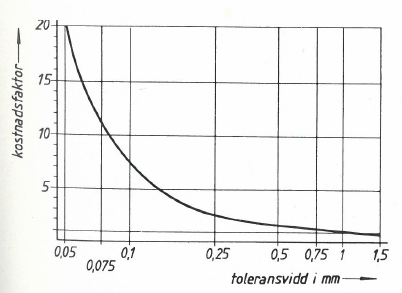
\includegraphics[width=0.4\paperwidth]{graphics/CostToleranceCausation}\caption{Tolerance widths (x-axis) and cost factor (y-axis). Adopted from \citealt{Lundkvist1997}\label{fig:CostToleranceCausation}}
\end{figure}

Engineering fit is defined by the dimensional difference of two assembled
components. Engineering fit can result in two cases, interference
or clearance. Interference is created when the cross sectional area
of a shaft is larger than the diameter of a hole. Clearance occurs
if the hole diameter is greater than the shaft diameter. When calculating,
interference and clearance are defined as grip $\bar{g}$ according
to equation \ref{eq:Interference}.\\
\begin{equation}
\bar{g}=\bar{d}_{h}-\bar{d}_{a}\label{eq:Interference}
\end{equation}

Interference fit can be assembled using two different methods, by
using bonded press fit or bonded shrink fit. To create an interference
fit, the shaft diameter must be greater than the hole diameter. Press
fit are assembled by applying a force which forces the shaft into
the hole. The weakest material of the components will slightly deform
but without losing the fit characteristics. The shrink fit is assembled
by either cooling the shaft, which will result in shrinkage, or by
heating the hole, which will result in expansion of the hole. As either
parts are experiencing dimensional changes due to change in temperature,
they are forced together. The parts will return to their normal dimensions
as they are no longer exposed to thermal conductivity and will generate
an interference fit.

\pagebreak{}

\section{Contact Mechanics}

Contact mechanics studies the deformation and stresses of a solid
which is in contact with another solid. The following formulation
of contact mechanics applies if one solid is a fixed rigid body.\\
The conditions of a contact system are defined by Signorini's contact
conditions \citealt{Stromberg2012}. The potential energy of the system
in function of a displacement vector is defined by\\
\begin{equation}
\Pi(\boldsymbol{d})=\frac{1}{2}\boldsymbol{d}^{T}\boldsymbol{Kd}-\boldsymbol{F}^{T}\boldsymbol{d},\label{eq:PotentialEnergySignorini's}
\end{equation}
where \textbf{K} is the stiffness matrix and \textbf{F} is the external
nodal force vector. The difference of the elastic energy within the
system and the external work results in the potential energy within
the system. The stage as which the lowest potential energy within
the system is the same stage which satisfies equilibrium.\\
\begin{equation}
\text{\ensuremath{\underset{\boldsymbol{d}}{\mathrm{min}}\:\Pi}(\ensuremath{\boldsymbol{d}})}\label{eq:PotentialEnergyEquilibrium}
\end{equation}
 Lowest potential energy within the system is defined by\\
\begin{equation}
\nabla\Pi(\boldsymbol{d})=\boldsymbol{Kd}-\boldsymbol{F}=0\label{eq:MINPotentialEnergy}
\end{equation}
\begin{figure}[H]
\begin{centering}
\includegraphics[width=0.4\paperwidth]{\string"graphics/Contact mechanics\string".eps}\caption{Elastic body kinematic constrained by a fixed rigid obstacle. Adopted
from \citealt{Stromberg2012}}
\par\end{centering}
\end{figure}
An obstacle is presented to restrict the elastic body to deform freely.
Kinematic constraints which prevents the body to penetrate the obstacle
are defined by\\
\begin{equation}
\boldsymbol{d}\boldsymbol{n}-g\leq0,\label{eq:KinematicConstraint}
\end{equation}
where $\boldsymbol{d}$ is displacement vector, $\boldsymbol{n}$
is normal direction vector of contact and $g$ is distance to the
obstacle in normal direction. The equation must be less or equal to
zero to meet the constraints i.e. the distance to the obstacle must
be greater or equal to the dislocation to have an operating contact.
The kinematic constraints can be defined for all contacts nodes by\\
\begin{equation}
\boldsymbol{C}_{N}\boldsymbol{d}-\boldsymbol{g}\leq0,\label{eq:GLOBALKinematicConstraint}
\end{equation}
where $\boldsymbol{C}_{N}$ is a transformation matrix of $\boldsymbol{n}$
and $\boldsymbol{g}$ is a vector of all initial gaps $g$.\\
The kinematic constraints can be included in the equilibrium principle
of the contact problem, i.e.\\
\begin{equation}
\text{\ensuremath{\begin{cases}
 \mathrm{\;\underset{\boldsymbol{d}}{min}\:}\Pi(\boldsymbol{d})\\
 \;\mathrm{s.t.}\;\boldsymbol{C}_{N}\boldsymbol{d}-\boldsymbol{g}\leq0 
\end{cases}}}\label{eq:EquilibriumPrinciple}
\end{equation}
The optimal solution of constrained optimization problems are given
by Karusch-Kuhn-Tucker conditions (KKT-conditions):\\
\begin{equation}
\ensuremath{\begin{cases}
\boldsymbol{Kd}-\boldsymbol{F}+\boldsymbol{C}_{N}^{T}\boldsymbol{P}_{N}^{A}=0\\
\boldsymbol{P}_{N}^{A}\geq0\\
\boldsymbol{C}_{N}\boldsymbol{d}-\boldsymbol{g}\leq0\\
\boldsymbol{P}_{N}^{A}\circ\left(\boldsymbol{C}_{N}\boldsymbol{d}-\boldsymbol{g}\right)=0
\end{cases}},\label{eq:LagrangeFormulation}
\end{equation}
where $\boldsymbol{P}_{N}^{A}$ is the contact force in normal direction
of the contact. The formulation of this problem is called Lagrange
formulation. A central distinction of Lagrangian formulation is that
it treats the conditions as additional equations and lagrange multipliers
$\boldsymbol{P}_{N}$ are interpreted as contact forces. The first
condition of the lagrange formulation defines the equilibrium state
of the system which is given by Signorini's contact conditions combined
with the contact force. The remaining conditions are given by KKT-conditions.
The first condition of KKT-conditions states that the contact force
must not be negative. The second KKT-condition states that the contact
distance must be greater or equal than the displacement in normal
direction i.e. the body can not penetrate the obstacle. The third
and last condition states that if there is no contact, the contact
force must be zero. The last condition also states that if there is
contact, the contact force must be greater than zero. \\
\\
Commercial FEA softwares approaches contact problems with an augmented
formulation of Lagrangian combined with either Uzawa's or Newton's
method. An augmented Lagrangian formulation includes the expression
of which stage equilibrium is satisfied and an equivalent formulation
of Signorini's condition, which is defined by

\begin{equation}
\begin{cases}
\;\underset{P_{N}^{A}}{\mathrm{max}}\:\left(d_{N}^{A}-g^{A}\right)P_{N}^{A}\\
\;s.t.\;P_{N}^{A}\geq0
\end{cases}\label{eq:AugmentedLagrangeFormulation}
\end{equation}
The contact force $P_{N}^{A}$ is equivalent to projection defined
by

\begin{equation}
\text{\ensuremath{\begin{cases}
 P_{N}^{A}=\left(P_{N}^{A}+r\left(d_{N}^{A}-g^{A}\right)\right)_{+}\\
 \;\mathrm{where}\;\mathbb{R_{+}}=\left\{  x:x\geq0\right\}  
\end{cases}}}\label{eq:ContactForceProjection}
\end{equation}
The foundation of Uzawa's and Newton's methods constitutes of the
projection of the contact force defined in (2.14). \citealt{Stromberg2012}\pagebreak{}

\section{Material Science and Engineering}

Material selection is a critical part of product development as it
has a direct impact of the performance of the product. Material selection
can also enable that tough requirements of the product/component is
met. It is essential that important material properties are prioritized
in order to optimize the function of a product or component. Material
properties can be categorized into general, mechanical, optical, thermal
and electrical, just to mention a few. Important material characteristics
regarding this thesis are defined below.

\subsection{Engineering Stress and Strain}

Stress, $\sigma$, within the material occurs when a force, $F$,
is acting on the cross-sectional area, $A$, according to equation
\ref{eq:Stress}. Engineering stress does only account for the initial
cross-sectional area, whereas the force can differentiate in a stress-strain
curve.

\begin{equation}
\sigma=\frac{F}{A}\label{eq:Stress}
\end{equation}

Strain, $\varepsilon$, is a result of an applied stress on the material.
If the applied tensile or compressive stress is large enough, the
material will either increase or decrease in length. Strain is defined
by the change in length, $\Delta l$, divided by the original length,
$l_{0}$, according to equation \ref{eq:Strain}.

\begin{equation}
\varepsilon=\frac{l_{i}-l_{0}}{l_{0}}=\frac{\Delta l}{l_{0}}\label{eq:Strain}
\end{equation}


\subsection{Hooke's Law}

Materials do not behave similarly when exposed to stress. A measurement
of a material\textquoteright s ability to withstand changes in length
when stress is applied was there for required to form a relationship.
Young\textquoteright s modulus $E$, named after the 18th-century
English scientist Thomas Young, defines such relationship. Hooke\textquoteright s
law defines the relationship between stress-strain-young\textquoteright s
modulus according to equations \ref{eq:Young's}.\citealt{Callister2011}

\begin{equation}
E=\frac{\sigma}{\varepsilon}\label{eq:Young's}
\end{equation}
\pagebreak{}

\subsection{Yield Stress}

Elastic deformation refers to the ability of a material to return
to its original form after being exposed to stress. If however, the
applied stress is large enough, the material will undergo permanent
deformation, also known as plastic deformation. The stress limit of
elastic deformation is determined by the proportional point $P$,
which is individual for each material. The proportional point $P$
is defined by the initial divergence from linearity of the stress-strain
curve. The initial divergence is very difficult to define and as a
consequence, yield stress/strength has been introduced. The yield
stress of a material is defined by the offset method. The method constructs
a parallel line to the linear stress-strain curve with an offset of
0.2\% strain. The stress corresponding to where the constructed line
intersects with the stress-strain curve is defined as the yield stress,
or the yield strength of a material, see Figure \ref{fig:YieldStress}.
As 0.2\% strain is almost negligible, the yield strength $\sigma_{y}$
is often referred to the stress limit which a material can withstand
without plastically deform. \citealt{Callister2011}

\begin{figure}[H]
\begin{centering}
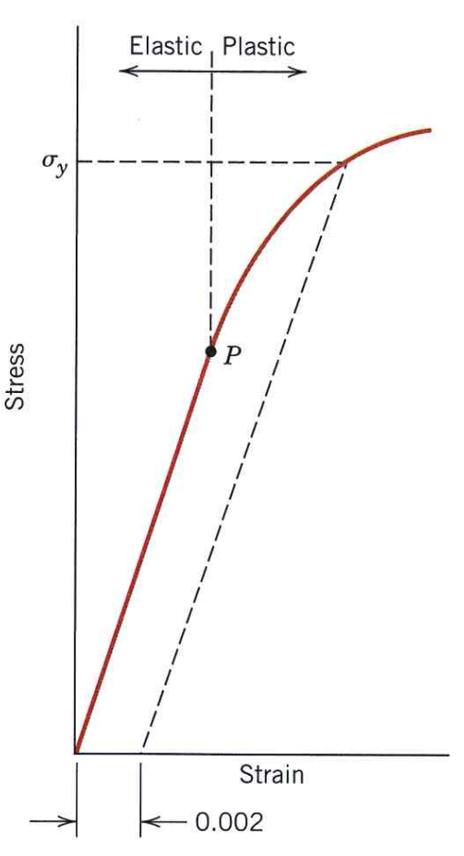
\includegraphics[height=0.3\paperheight]{graphics/YieldStress}\caption{Stress-strain curve with offset-method.\label{fig:YieldStress} Adopted
from \citealt{Callister2011}}
\par\end{centering}
\end{figure}
\pagebreak{}

\subsection{Strain Hardening}

Strain hardening, or work hardening, is the hardening which increases
the strength and decreases the ductility of a material which experience
strain. Strain hardening can be defined in an engineering stress-strain
curve or in a true stress-strain curve. An engineering stress-strain
curve is designated by the computation with a constant area. A constant
cross-sectional area generates a curve which displays that no additional
stress is required to fracture as the stress reached the material's
ultimate tensile.

A true stress-strain curve defines stress and strain accordingly,

\begin{equation}
\sigma_{true}=\frac{F}{A_{i}}\label{eq:TrueStress}
\end{equation}

\begin{equation}
\varepsilon_{true}=\mathrm{ln}(\frac{L_{i}}{L_{0}})\label{eq:TrueStrain}
\end{equation}

True stress and strain can be defined in relation to engineering strain
can be expressed according to the definitions \ref{eq: TrueStress2}
\& \ref{eq:TrueStrain2},

\begin{equation}
\sigma_{true}=\sigma(1+\varepsilon)\label{eq: TrueStress2}
\end{equation}

\begin{equation}
\varepsilon_{true}=\mathrm{ln}(1+\varepsilon)\label{eq:TrueStrain2}
\end{equation}

The definition of stress and strain separates the true and engineering
approach. True stress and true strain takes the instantaneous values
of the cross-sectional area $A_{i}$ and the length $l_{i}$ into
account according to the definitions expressed in eq \ref{eq:TrueStress}
and equation \ref{eq:TrueStrain}. The engineering stress-strain only
considers the original cross-sectional area for stress and the final
strain for strain. The result of this is two different looking stress-strain
curves whereas true stress-strain will be conducted in this thesis,
see Figure \ref{fig:True-Stress-Strain-curve}.

Strain hardening occurs as the stress exceeds the yield stress. The
material plastically deformations at stresses higher than the material's
yield strength. Plastic deformation permanently deforms the material,
previously called strain hardening. The stress-strain relation of
strain hardening can be displayed using a tangent modulus. Tangent
modulus can be defined as bilinear or multilinear. A bilinear tangent
modulus consists of only one linear tangent between two points. Multilinear
consists of several linear tangents. Bilinear tangent modulus can
be useful when the strain hardening behavior is unknown but e.g. yield
stress and Ultimate tensile stress is known.\pagebreak{}

To calculate the tangent modulus between the point of yield stress
and the point of ultimate tensile stress, four coordinates are required.
$\sigma_{y}$ yield stress, $\varepsilon_{y}$ strain at yield stress,
$\varepsilon_{UTS_{true}}$ strain at true ultimate tensile stress
and $\sigma_{UTS_{true}}$ true ultimate tensile stress. The coordinates
are obtained accordingly,

\[
\sigma_{y}=\text{Given\:value\:of\:yield\:stress\:[MPa]}
\]

\[
\varepsilon_{y}=\frac{\sigma_{y}}{E}
\]

\[
\varepsilon_{UTS_{true}}=\mathrm{ln}(1+\frac{\text{elongation\%}}{100})
\]

\[
\sigma_{UTS_{true}}=\sigma_{UTS}(1+\varepsilon_{UTS_{true}})\:\text{[MPa]},
\]
where $E$ is the Young's modulus. The slope of the tangent modulus
can then be calculated by equation \ref{eq:TangentModulusCalc},

\begin{equation}
E_{t}=\frac{\left(\sigma_{UTS_{true}}-\sigma_{y}\right)}{\left(\varepsilon_{UTS_{true}}-\varepsilon_{y}\right)}\label{eq:TangentModulusCalc}
\end{equation}
\begin{figure}[H]

\begin{centering}
\includegraphics[width=0.55\paperwidth]{\string"graphics/Comparison Stress Strain Curve\string".eps}\caption{True Stress-Strain curve and Engineering Stress-Strain curve comparison
and accompanying explanation of bilinear tangent modulus \label{fig:True-Stress-Strain-curve}}
\par\end{centering}
\end{figure}

\pagebreak When a stress larger than the yield strength of a material
is removed, partial elastic recovery of the total deformation will
occur. The result of plastic deformation will not affect the material\textquoteright s
ability to still elastically deform, but as an already plastically
deformed material. The amount of strain a material can experience
is determined by the ductility of a material.

\subsection{Ductility}

Ductile materials can deform to a certain rate without fracturing.
Ductile materials are favorable when the design of the component requires
forming operations. Ductility is defined in percent as elongation
according to the equation \ref{eq:Elongation}.

\begin{equation}
\%EL=\left(\frac{l_{f}-l_{o}}{l_{0}}\right)100\label{eq:Elongation}
\end{equation}

The opposite of ductile is brittle. The atoms in brittle materials
are bonded and structured in such way to prevent strain. Fracture
in brittle material can there for be sudden and unexpected, see Figure
\ref{fig:Ductility}. \citealt{Callister2011}

\begin{figure}[H]
\begin{centering}
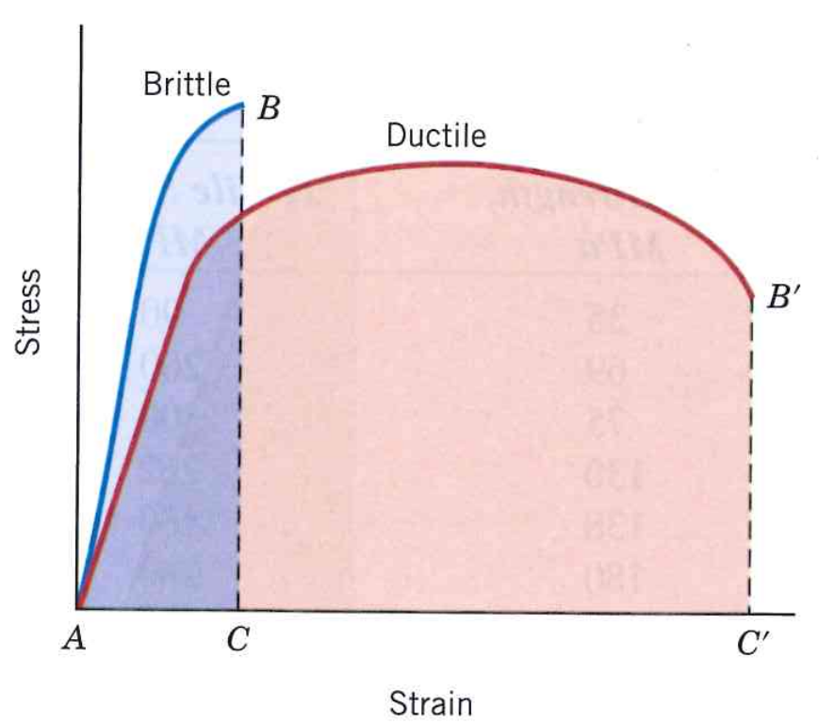
\includegraphics[width=0.35\paperwidth]{graphics/Ductility}\caption{Characteristics of a brittle and ductile material in a Stress-strain
curve.\label{fig:Ductility} Adopted from \citealt{Callister2011}}
\par\end{centering}
\end{figure}


\chapter{Method}

\textit{This chapter provides an overview and a description of the
carried out method used to achieve a valid result.}

\section{Concept and Evaluation Study}

The objective of this thesis was to design and evaluate spring element
based of given requirements. Concepts were generated and then screened
to obtain a final concept which had the most potential to meet each
requirement. The final concept was then evaluated using finite element
analysis.

\subsection{Finite Element Analysis}

The finite element method (FEM) is a numerical method used to perform
finite element analysis of any given physics problem. Typical physics
problem includes structural analysis, heat transfer, fluid flow and
electromagnetic potential. The problems can be defined in partial
differential equations (PDE). To be solved, the analytic solution
requires boundary values of the PDE, which are rarely obtained. Finite
element formulation consists of a system of algebraic equations instead.
To simplify the solution of the system consisting of unknown numerical
values, it is subdivided into smaller systems also known as finite
elements. Finite equations consisting of numerical values simplifies
the calculations, but the number of equations to solve is increased.
By utilizing the computation time of a computer, the system can be
solved effectively, which is performed in several modern softwares.
The solution of each equation can then be assembled into a larger
system which defines the entire problem.\citealt{Logan2012}

Finite element analysis is performed in this thesis to find the solutions
regarding the given requirements. The solutions determined if the
spring element met each requirement.

\section{Validity and Reliability}

Validity is achieved by performing a finite element analysis, which
is a commonly used method to obtain results of stresses, strains and
reaction forces in a given problem. Reliably results are achieved
by simulating worst cases which represents scenarios with the least
favorable parameters such as, dimensions, material properties and
friction coefficients. A mesh independence study is performed to achieve
a mesh which provides a result with high accuracy. Contacts are analyzed
using Contact Status to ensure no significant interpenetration of
surfaces would occur.

\chapter{Analysis}

\textit{A thorough presentation of the simulation analysis will be
conducted in Chapter 4.}

\section{ANSYS Workbench}

The finite element analysis in this thesis was performed using ANSYS
Mechanical 18.2. The simulation consisted of three components, the
spring element concept, the armature and the valve body. Symmetrical
planes were evaluated of each component's geometry to simplify the
simulation and decrease the time required to solve the problem. ANSYS
consists of multiple analysis systems, which is chosen depending on
the problem. Static structural is an analysis system which was chosen
for the problem in this thesis. Static structural determines stresses,
strains and reaction forces caused by steady loading i.e., loads that
with respect to time varies slowly. Static structural allows linear
or nonlinear behaviors, example of nonlinearity behaviors are large
deflections, plasticity, friction coefficient and contacts. This thesis
consisted of a nonlinear contact problem which was solved using an
implicit solver. The solver consisted of an unsymmetrical Newton-Raphson
method.

ANSYS allows multiple number of load steps. Each load step has a virtual
time unit of 1. Each load step also consists of points at which solutions
are computed, in ANSYS these points are called substeps. The amount
of substeps can manually be controlled to obtain convergence. Convergence
occurs when the residual, the difference between the external and
internal force, is less than the convergence criterion. Error is inherent
in nonlinear analysis, convergence criterion is basically the allowance
of error, usually in percentage.

\begin{table}
\begin{centering}
\begin{tabular}{|c|c|c|}
\hline 
Parameter & Error $\epsilon=\sqrt{\int_{\Omega}\left(u_{e}-u_{a}\right)^{2}d\Omega}$ & Efficiency\tabularnewline
\hline 
\hline 
$\delta_{1}$ & 0.14 & 97\%\tabularnewline
\hline 
$\delta_{2}$ & 0.16 & 96\%\tabularnewline
\hline 
\end{tabular}\caption{Some table}
\par\end{centering}
\end{table}

\pagebreak{}

\section{Some tricky stuff}

\begin{equation}
\bm{\Phi}:=\begin{bmatrix}\varphi_{1} & 0 & 0 & \varphi_{2} & 0 & 0 & \cdots\\
0 & \varphi_{1} & 0 & 0 & \varphi_{2} & 0 & \cdots\\
0 & 0 & \varphi_{1} & 0 & 0 & \varphi_{2} & \cdots
\end{bmatrix}\label{eq:FiDiscrete}
\end{equation}

This matrix needs to be stretched a bit otherwise it's very dense

\renewcommand*{\arraystretch}{1.5} 

\[
\bm{J}(\xi,\eta,\zeta)=\begin{bmatrix}\dfrac{\partial x_{h}}{\partial\xi} & \dfrac{\partial y_{h}}{\partial\xi} & \dfrac{\partial z_{h}}{\partial\xi}\\
\dfrac{\partial x_{h}}{\partial\eta} & \dfrac{\partial y_{h}}{\partial\eta} & \dfrac{\partial z_{h}}{\partial\eta}\\
\dfrac{\partial x_{h}}{\partial\zeta} & \dfrac{\partial y_{h}}{\partial\zeta} & \dfrac{\partial z_{h}}{\partial\zeta}
\end{bmatrix}
\]
\renewcommand*{\arraystretch}{1}
\begin{center}
 \resizebox{\textwidth}{!}{%%
\begin{tabular}{c|c|c}
State of stress & Boundary Conditions & von Mises Equations\tabularnewline
\hline 
 &  & \tabularnewline
General 3D & No restrictions & $\sigma_{v}=\sqrt{\frac{1}{2}\left[\left(\sigma_{x}-\sigma_{y}\right)^{2}+\left(\sigma_{y}-\sigma_{z}\right)^{2}+\left(\sigma_{z}-\sigma_{x}\right)^{2}+6\left(\sigma_{xy}^{2}+\sigma_{yz}^{2}+\sigma_{zx}^{2}\right)\right]}$\tabularnewline
General plane stress (2D) & $\sigma_{z}=\sigma_{yz}=\sigma_{zx}=0$ & $\sigma_{v}=\sqrt{\sigma_{x}^{2}-\sigma_{x}\sigma_{y}+\sigma_{y}^{2}+3\sigma_{xy}^{2}}$\tabularnewline
\end{tabular}}
\par\end{center}

\begin{algorithm}[h]
\begin{lstlisting}[language=Matlab,basicstyle={\ttfamily},breaklines=true,keywordstyle={\color{blue}},frame=single]
for iel = 1:nele       % Loop over all elements
   inod = nodes(iel,:) % Current element nodes
   % Compute Sk
   % Compute fk

   % Assembly
   S(inod,inod) = S(inod,inod) + Sk;
   F(inod) = F(inod) + fk;
end
\end{lstlisting}

\caption{Element loop}
\end{algorithm}

\pagebreak{}

\section{Some more analys}

\lipsum[1-2]\pagebreak{}

\chapter{Results}

\textit{This chapter presents the result of concept development and
the result of the final concept evaluation using finite element analysis.}

\section{Final Concept}

\lipsum[1-2]

\chapter{Discussion}

\textit{Discussion of implications and lessons learned regarding this
problem are presented in Chapter 7.}

\section{Implications}

Implications, uncertainties and suggestions of improvement are presented
in this section.

\subsection{Brainstorming and Pugh Matrix}

To fully utilize concept generation, several participants are required.
In this thesis, brainstorming was solely performed by the author himself.
This restricts the method and the benefits of having several creative
participants which combined creates concepts. Several participants
bring additional viewpoints of a given problem which may result in
a creative solution.

Concepts had to be eliminated to obtain a final concept. The elimination
had to be performed with several requirements unanswered. Gut feeling
and concept comparision of several non critical requirements determined
the final concept. This may have resulted in a concept with not the
best potential of meeting each requirement being evaluated using FEA.

The most optimal would have been having several participants performing
concept generation and by evaluating several concepts using FEA.

\subsection{Friction Coefficient}

An essential area in this thesis was contact mechanics. To ensure
a reliable result of the simulation, the friction coefficients are
extremely crucial. To obtain true friction coefficients, the specific
alloying materials used with corresponding surface roughness achieved
by respective manufacturing methods had to be produced. These values
haven't previously been produced and delivery time of desired material
samples prevented an experimental evaluation to be performed. Instead,
a general value of friction coefficients of the material combinations
was used. These general values didn't take alloying materials in account
and categorized surface roughness by dry or lubricated surfaces and
not by manufacturing methods. This results in an uncertain value of
friction coefficients which may affect the final result.\pagebreak{}

\subsection{Simulated Spring Element Model}

To achieve a true result of the simulation, the cad model of the spring
element must be similar to a manufactured spring element. A manufactured
spring element using deep drawing experiences dilution at the bend
radius. The 3D model in NX was not modeled with dilutions but with
an uniform material thickness. This results in a simulation result
with increased solid mechanics of the spring element. If the dilution
is critical, the result of the simulations may have resulted differently.

\subsection{Computation Time}

Computation time has been a critical parameter in this thesis. The
computation time couldn't be decreased due to the model consisting
of a 3D nonlinear contact problem which prevented simulation in 2D.
Simulations requiring five hours each limits an effective work. This
is partially the cause of a single concept could just be evaluated
using finite element analysis.

\section{Lessons Learned}

To fully evaluate the feasibility of an additional component manufactured
using a deep drawing process, the friction coefficient must be known.
A simulation using worst case 1 dimensions with the upper range of
friction coefficient of steel - steel contact provided a different
result. Instead of the armature being disassembled, which was the
main purpose of worst case 1, the valve body was disassembled. This
displays the significance of friction coefficient. An increased friction
coefficient may not require a large contact area to maintain assembly
during e.g, transportation.

Spring functionality was a high priority when concepts were evaluated.
Spring functionality did not cause any requirements not to be met.
The results displayed however, that contact statuses and friction
coefficient to be the cause of an unmet requirement. This may has
caused an incorrect priority of achieving the greatest spring functionality
instead of achieving larger contact statuses. Concepts might have
been eliminated by an incorrect prioritization.

The difficulty using an additional component is achieving two different
press fits of a single component, an external and an internal press
fit. This entails implications of counteracting press fits, which
is not desired. A suggestion of future solutions is to generate solutions
which do not include an additional component. Instead, design changes
of the already existing armature or valve body should be evaluated.
If the interface of the armature enables spring functionality, only
one press fit is required and tolerances of the valve body could potentially
be increased.

\chapter{Conclusions}

\textit{This chapter summarizes if each requirement was fulfilled
and which issues were answered.}

\section{Requirements Summary}

It could be concluded that the solid mechanics of the spring element
was approved by stresses which not exceeded the material's ultimate
tensile strength. A highly prioritized requirement stated that no
critical deformation of the valve body's inner surfaces and the armature's
threads must occur. Deformation evaluation was performed by a comparison
to the surfaces tolerances, which determined that the deformations
could be neglected. The escape passage was evaluated at the least
favorable dimensions but, compared to the pd-restriction, it yielded
a safety factor of 1.8. Safety factor of 1.8 defines the capacity
ratio of not causing a pressure drop within the pilot stage. Safety
factor 1.8 was computed with the least favorable parameters, which
according to the normal distribution of manufacturing rarely will
be obtained.

Required assembly forces of the armature and the valve body in both
worst cases were computed to a maximum of 72 N, which considering
an automated assembly process is approved. The disassembly force of
the valve body in worst case 1 was computed to 32 N, which compared
to the mass of the valve and the gravitational force yielded a safety
factor of 105. A safety factor of 105 doesn't include which g-forces
the valve experiences during transportation or assembly, which prevents
the disassembly force of worst case 1 to be approved without a more
in depth evaluation. Worst case 2 required no disassembly force to
disassemble the armature, which without a further evaluation could
be determined not approved. Significant decrease in contact status
of the internal press fit as the armature was assembled was the decisive
cause of no disassembly force required.\pagebreak{}

\section{Answered Issues}
\begin{itemize}
\item How should the spring element be designed to meet the requirements?\\
- Since each requirement wasn't fulfilled by the spring element implementation,
the first issue of how a spring element should be designed to meet
each requirement could not be answered
\item How should the solid mechanics of the spring element be evaluated?\\
- With a finite element analysis which with high accuracy and efficiency
could provide data regarding each requirement.
\item Which material is suitable for such spring element in such conditions?\\
- SSAB's Form 03 which is a soft steel alloy recommended for deep
drawing process. The material didn't reach fracture stresses during
spring element evaluation which implies the material could sustain
such conditions it experienced.
\end{itemize}

\chapter{Future Work}
\begin{itemize}
\item Produce or order data of precise friction coefficients with correct
surface roughness and material
\item Evaluate the feasibility of implementing spring functionality of the
armature, which reduces the press fits to solely one
\end{itemize}
%\markboth{Bibliography}{Bibliography}

%\markboth{\spacedlowsmallcaps{\chaptername}\ \spacedlowsmallcaps{\thechapter}.\ #1}{}
\markboth{Bibliography}{Bibliography}

\printbibliography[heading=bibintoc]


\appendix

\chapter{Mesh Independence Study \label{chap:Mesh-Independence-Study}}

\lipsum[1-3]
\end{document}
